% =====================================================================
%  MiniVPN -- Operating System Lab Synopsis
%  Compile:  pdflatex synopsis.tex   (run twice for references)
%  Needs jiit-logo.png in the same folder.
% =====================================================================
\documentclass[12pt,a4paper]{article}

\usepackage[margin=1in]{geometry}
\usepackage{graphicx}
\usepackage{setspace}
\usepackage{enumitem}
\usepackage{booktabs}
\usepackage{tabularx}
\usepackage{xcolor}
\usepackage{tikz}
\usetikzlibrary{positioning,arrows.meta,shapes.geometric,fit}
\usepackage[hidelinks]{hyperref}

\setstretch{1.25}
\setlist{itemsep=2pt,topsep=4pt}

% Running header and page number (no extra package needed)
\makeatletter
\def\ps@project{%
  \def\@oddhead{\small MiniVPN -- OS Lab Synopsis\hfill JIIT, Noida}%
  \let\@evenhead\@oddhead
  \def\@oddfoot{\hfil\thepage\hfil}%
  \let\@evenfoot\@oddfoot}
\makeatother
\pagestyle{project}

% ---------------------------------------------------------------------
%  Front-page details -- edit here
% ---------------------------------------------------------------------
\newcommand{\projecttitle}{MiniVPN: A Secure Self-Hosted Virtual Private Network Built on Linux Kernel Interfaces}
\newcommand{\doctype}{Operating System Lab Synopsis}
\newcommand{\semester}{Semester 5}

\begin{document}

% =========================== FRONT PAGE ==============================
\begin{titlepage}
\centering
{\Large\bfseries BACHELOR OF TECHNOLOGY\par}
\vspace{1.2cm}

\includegraphics[width=4.2cm]{jiit-logo.png}\par
\vspace{0.6cm}
{\large Jaypee Institute of Information Technology, Noida\par}
\vspace{1.4cm}
{\LARGE\bfseries \projecttitle\par}
\vspace{1.2cm}
{\Large \semester\par}
\vspace{0.4cm}
{\Large\bfseries \doctype\par}
\vfill
\begin{minipage}[t]{0.52\textwidth}
\raggedright
{\large\bfseries Made By:}\\[6pt]
Sansriti Mishra \hfill 2401030293\\
Mokshi Mittal \hfill 2401030326\\
Sanvi Dhingra \hfill 2401030312
\end{minipage}%
\hfill
\begin{minipage}[t]{0.38\textwidth}
\raggedleft
{\large\bfseries Submitted To:}\\[6pt]
Dr. Sayani Ghoshal\\
Dr. Vikash\\
Dr. Tanvi Gautam
\end{minipage}
\vspace{1.5cm}

{\large Department of Computer Science \& Engineering and IT\par}
\end{titlepage}

% ============================ BODY ===================================

\section{Introduction}
A \emph{Virtual Private Network} (VPN) joins machines that are physically spread across
the Internet into one private network. Packets between them are encrypted and
authenticated, so an observer on the path cannot read or modify them. Products such as
OpenVPN and WireGuard are widely used, but they are large codebases. To a student they
look like black boxes.

\textbf{MiniVPN} is a VPN written from scratch in C for Linux. The project builds the
complete stack ourselves: the virtual network interface, the event loop, the session
table, the cryptographic handshake and the management tools. Each part is a direct
application of an operating-system concept: virtual devices, \texttt{ioctl}-based kernel
configuration, I/O multiplexing with \texttt{epoll}, signals and timers as file
descriptors, privilege separation, inter-process communication and file locking.

\section{Problem Statement}
Small teams and labs need a private network that connects laptops, servers and offices.
Existing solutions are either hosted services (which route traffic through a third
party) or complex tools that are hard to configure and audit. The goal is a VPN that is:
\begin{itemize}
  \item \textbf{Secure:} modern authenticated encryption, forward secrecy, replay and spoofing protection;
  \item \textbf{Manageable:} one command to add a device and instant revocation when someone leaves;
  \item \textbf{Small and understandable:} a few thousand lines of C that show how the kernel
        networking stack, processes and file descriptors cooperate.
\end{itemize}

\section{Objectives}
\begin{enumerate}
  \item Create and configure a Linux TUN virtual network device from user space using
        \texttt{/dev/net/tun} and \texttt{ioctl} calls (address, netmask, MTU, routes).
  \item Design a single-threaded, event-driven server and client using \texttt{epoll},
        with signals handled through \texttt{signalfd} and periodic work through \texttt{timerfd}.
  \item Encapsulate IP packets inside UDP and protect them with X25519 key exchange and
        ChaCha20-Poly1305 authenticated encryption.
  \item Apply OS security principles: drop root privileges after setup, restrict the
        control socket with \texttt{SO\_PEERCRED}, and update files atomically with
        \texttt{flock}, \texttt{fsync} and \texttt{rename}.
  \item Build a management tool (CLI and web dashboard) that talks to the running daemon
        over a Unix-domain socket.
  \item Verify correctness with unit tests and end-to-end tests that run in isolated
        Linux network namespaces.
\end{enumerate}

\section{Proposed System Architecture}

\begin{figure}[h]
\centering
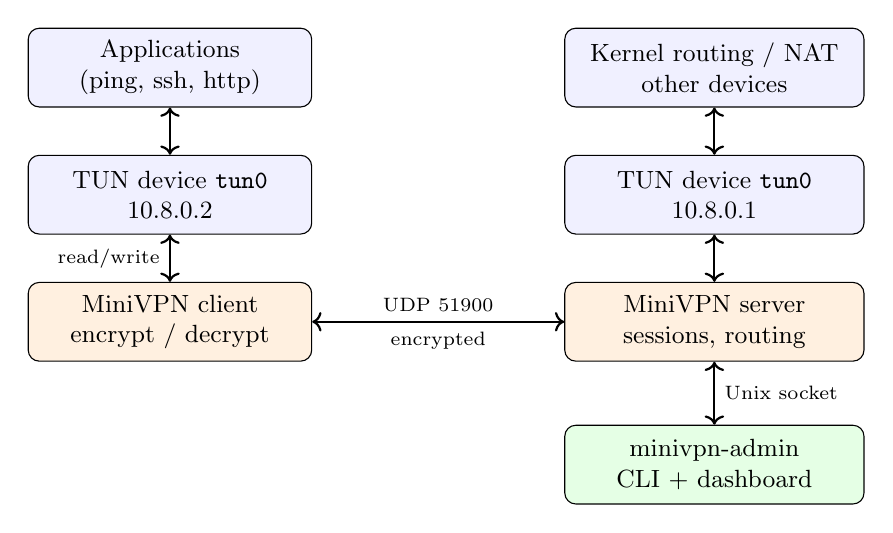
\begin{tikzpicture}[
  box/.style={draw,rounded corners,align=center,minimum height=1cm,font=\small,fill=blue!6},
  arr/.style={-{Stealth},thick}]
  \node[box,minimum width=3.6cm] (app) {Applications\\(ping, ssh, http)};
  \node[box,below=0.6cm of app,minimum width=3.6cm] (tun) {TUN device \texttt{tun0}\\10.8.0.2};
  \node[box,below=0.6cm of tun,minimum width=3.6cm,fill=orange!12] (cli) {MiniVPN client\\encrypt / decrypt};
  \node[box,right=3.2cm of cli,minimum width=3.8cm,fill=orange!12] (srv) {MiniVPN server\\sessions, routing};
  \node[box,above=0.6cm of srv,minimum width=3.8cm] (stun) {TUN device \texttt{tun0}\\10.8.0.1};
  \node[box,above=0.6cm of stun,minimum width=3.8cm] (lan) {Kernel routing / NAT\\other devices};
  \node[box,below=0.8cm of srv,minimum width=3.8cm,fill=green!10] (adm) {minivpn-admin\\CLI + dashboard};
  \draw[arr,<->] (app) -- (tun);
  \draw[arr,<->] (tun) -- node[left,font=\scriptsize]{read/write} (cli);
  \draw[arr,<->] (cli) -- node[above,font=\scriptsize]{UDP 51900}
                          node[below,font=\scriptsize]{encrypted} (srv);
  \draw[arr,<->] (srv) -- (stun);
  \draw[arr,<->] (stun) -- (lan);
  \draw[arr,<->] (adm) -- node[right,font=\scriptsize]{Unix socket} (srv);
\end{tikzpicture}
\caption{High-level architecture of MiniVPN}
\end{figure}

An application on a device sends an ordinary IP packet. The kernel routes it to the
virtual interface \texttt{tun0}. Instead of reaching a wire, the packet is delivered to
the MiniVPN client process, which reads it with \texttt{read()}. The client encrypts it,
wraps it in a UDP datagram and sends it to the server. The server authenticates and
decrypts it, checks that the source address belongs to that device, and writes it into
its own TUN device. From there the kernel forwards it to its destination. Replies take
the reverse path.

\section{Operating-System Concepts Applied}
\begin{tabularx}{\textwidth}{@{}lX@{}}
\toprule
\textbf{Concept} & \textbf{Use in MiniVPN}\\
\midrule
Virtual devices & \texttt{open("/dev/net/tun")} + \texttt{ioctl(TUNSETIFF)} creates a network interface backed by a file descriptor\\
Kernel configuration & \texttt{SIOCSIFADDR}, \texttt{SIOCSIFNETMASK}, \texttt{SIOCSIFMTU}, \texttt{SIOCADDRT} ioctls; \texttt{/proc/sys/net/ipv4/ip\_forward}\\
I/O multiplexing & One thread waits on TUN, UDP, signal, timer and control fds with \texttt{epoll\_wait}\\
Signals & \texttt{sigprocmask} + \texttt{signalfd}: \texttt{SIGHUP} reloads, \texttt{SIGTERM} shuts down cleanly\\
Timers & \texttt{timerfd} drives keepalives, retransmission, rekeying and session expiry\\
Privilege separation & Start as root to create the device, then \texttt{setgid}/\texttt{setuid} to an unprivileged user\\
IPC & Unix-domain stream socket for \texttt{status}, \texttt{reload}, \texttt{kick}; caller checked with \texttt{SO\_PEERCRED}\\
File system & Advisory locking (\texttt{flock}) and crash-safe updates (write temp, \texttt{fsync}, \texttt{rename})\\
Process isolation & Linux network namespaces simulate several machines on one computer for testing\\
Service management & systemd units with sandboxing options\\
\bottomrule
\end{tabularx}

\section{Methodology}
\begin{enumerate}
  \item \textbf{TUN layer:} open and configure the virtual interface; read and write raw IPv4 packets.
  \item \textbf{Transport:} non-blocking UDP socket; define a compact binary packet format.
  \item \textbf{Event loop:} integrate all file descriptors into \texttt{epoll}; add \texttt{signalfd} and \texttt{timerfd}.
  \item \textbf{Security:} one-round-trip handshake (HELLO / WELCOME) with HMAC authentication,
        HKDF key derivation and ChaCha20-Poly1305 data channel; 1024-entry anti-replay window.
  \item \textbf{Server features:} per-device session table, fixed tunnel addresses, roaming,
        keepalives, rekeying, live revocation through the control socket.
  \item \textbf{Management:} Python administration CLI and web dashboard; device registry and configuration files.
  \item \textbf{Testing:} unit tests against published RFC test vectors and end-to-end tests in network namespaces;
        AddressSanitizer and UBSan builds to catch memory errors.
\end{enumerate}

\section{Tools and Technologies}
\begin{tabularx}{\textwidth}{@{}lX@{}}
\toprule
Language & C (C11) for the daemon, Python 3 (standard library) for administration\\
Libraries & OpenSSL \texttt{libcrypto} (X25519, ChaCha20-Poly1305, HMAC-SHA256, Ed25519)\\
Platform & Linux (Ubuntu on WSL2 for development)\\
Build and debug & GCC, GNU Make, GDB, AddressSanitizer, \texttt{tcpdump}, \texttt{ip netns}\\
Packaging & systemd service units, Debian \texttt{.deb} package\\
\bottomrule
\end{tabularx}

\section{Expected Outcomes}
\begin{itemize}
  \item A working VPN server and client that carry real traffic (ping, SSH, file transfer) between devices.
  \item Encrypted traffic on the wire: no plaintext visible in a packet capture.
  \item Instant enforcement of administrative actions (disable, revoke, kick) without restarting the server.
  \item Automatic recovery from network changes: reconnect, roaming and NAT keepalives.
  \item A test suite that demonstrates each OS and networking mechanism.
\end{itemize}

\section{Work Plan}
\begin{tabularx}{\textwidth}{@{}lX@{}}
\toprule
\textbf{Phase} & \textbf{Activity}\\
\midrule
Week 1--2 & Study TUN/TAP, \texttt{ioctl}, \texttt{epoll}; build a plaintext tunnel between two namespaces\\
Week 3--4 & Packet format, handshake and encrypted data channel; anti-replay window\\
Week 5--6 & Multi-device server, session table, signals, timers, privilege drop\\
Week 7--8 & Control socket, administration CLI and dashboard\\
Week 9--10 & Testing, sanitizers, packaging, documentation and report\\
\bottomrule
\end{tabularx}

\section*{References}
\begin{enumerate}[label={[\arabic*]}]
  \item M. Kerrisk, \emph{The Linux Programming Interface}, No Starch Press, 2010.
  \item A. Silberschatz, P. B. Galvin, G. Gagne, \emph{Operating System Concepts}, 10th ed., Wiley, 2018.
  \item Linux kernel documentation, \emph{Universal TUN/TAP device driver}, \url{https://docs.kernel.org/networking/tuntap.html}.
  \item J. A. Donenfeld, ``WireGuard: Next Generation Kernel Network Tunnel,'' NDSS, 2017.
  \item Y. Nir, A. Langley, \emph{ChaCha20 and Poly1305 for IETF Protocols}, RFC 8439, 2018.
  \item A. Langley, M. Hamburg, S. Turner, \emph{Elliptic Curves for Security}, RFC 7748, 2016.
  \item H. Krawczyk, P. Eronen, \emph{HMAC-based Extract-and-Expand Key Derivation Function (HKDF)}, RFC 5869, 2010.
\end{enumerate}

\end{document}
